In this section we build on hyperbolicity, establishing mixing properties using Theorem \ref{thm:katok-strelcyn}.

\begin{thm}
\label{thm:mixingOTM}
The map $H: \tor \to \tor$ is Bernoulli with respect to the Lebesgue measure.
\end{thm}

\subsection{Nature of local manifolds}

Noting that \textbf{(KS1-2)} were shown in \cite{myers_hill_exponential_2022}, by Theorem \ref{thm:katok-strelcyn}, local unstable and stable manifolds $\gamma_u(z), \gamma_s(z)$ exist at a.e. $z$. By definition, for any $\zeta,\zeta' \in \gamma_u(z)$
\begin{equation}
    \label{eq:unstableManifold}
    \mathrm{dist}(H^{-n}(\zeta),H^{-n}(\zeta')) \rightarrow 0
\end{equation} 
as $n \rightarrow \infty$. Similarly for any $\zeta,\zeta' \in \gamma_s(z)$
\begin{equation}
    \label{eq:stableManifold}
    \mathrm{dist}(H^{n}(\zeta),H^{n}(\zeta')) \rightarrow 0
\end{equation}
as $n\rightarrow \infty$.
Piecewise linearity of $H$ ensures that these local manifolds are line segments containing $z$, aligned with some vector $v = (v_1,v_2)^T$ of \emph{gradient} $v_2/v_1$. The following two lemmas establish bounds on their gradients when mapped under $H$ and its inverse.

\begin{lemma}
\label{lemma:OTMalignment}
For almost every $z$, there exists $m,n \in \mathbb{N}$ such that $H^{m}(\gamma_u(z))$ contains a line segment in $\sigma$ aligned with some $v\in \mathcal{C}$, and $H^{-n}(\gamma_s(z))$ contains a line segment in $\sigma'$ aligned with some $v' \in \mathcal{C}'$.
\end{lemma}

\begin{proof}
By definition of the $\sigma_j, \sigma_j'$, we have that $\sigma_j = H(\sigma_j')$ for $j=1,4$, and $\sigma_j = H^2(\sigma_j')$ for $j=2,3$. For almost every $z$ the number $m = \min \{ k \geq 1 \,| \, H^k(z) \in \sigma \}$ is well defined, as is the cocycle $DH_z^m$. On some portion of $\gamma_u(z)$ around $z$, the cocycle $DH_z^m$ will be constant so that the portion maps to some line segment $\Gamma$ under $H^m$. Hence $H^{m}(\gamma_u(z))$ contains a segment $\Gamma$ in $\sigma$, aligned with some vector $v$. Now if $\Gamma$ lies in $\sigma_1$, its preimage is a segment in $\sigma_1'$ aligned with the vector $M_1^{-1}v$. Now to satisfy (\ref{eq:unstableManifold}), $M_1^{-1}v$ must lie in some stable cone $\mathcal{C}_s'$ which contains all the stable eigenvectors of matrices in $\mathcal{M}'$ and none of the unstable eigenvectors. Hence $v \in M_1 \mathcal{C}_s'$. Similarly if $z\in \sigma_4$ then $v \in M_4 \mathcal{C}_s'$, if $z\in \sigma_2$ then $v \in M_2 M_3 \mathcal{C}_s'$, and if $z\in \sigma_3$ then $v \in M_3M_2 \mathcal{C}_s'$. Such a stable cone $\mathcal{C}_s'$ is given by $\{(v_1,v_2)\neq 0 \,|\, |v_2| \geq |v_1|\}$; one can verify that $M\mathcal{C}_s' \subset \mathcal{C}$ for each $M \in \{ M_1, M_4, M_2M_3, M_3M_2 \}$, verifying $v\in \mathcal{C}$. The argument for $v'\in \mathcal{C}'$ is entirely analogous.
\end{proof}

The expanding and invariance properties of the cone $\mathcal{C}$ formed from $\mathcal{M}$ will be key to growing the images of unstable manifolds. We can ensure stronger expansion by refining the cone, defining $\mathcal{C}_+,\mathcal{C}_-\subset \mathcal{C}$ by
% \begin{itemize}
%     \item $ 3\,|v_1| \geq |v_2| \geq \varphi \,|v_1|$, $v_1v_2>0$ over $\mathcal{C}_+$,
%     \item $ 3\,|v_1| \geq |v_2| \geq \varphi \,|v_1|$, $v_1v_2<0$ over $\mathcal{C}_-$.
% \end{itemize}
\begin{enumerate}[label={($\mathcal{C}_{+}$)}]
    \item $ 3\,|v_1| \geq |v_2| \geq \varphi \,|v_1|$, $v_1v_2>0$,
\end{enumerate}
\begin{enumerate}[label={($\mathcal{C}_{-}$)}]
    \item $ 3\,|v_1| \geq |v_2| \geq \varphi \,|v_1|$, $v_1v_2<0$.
\end{enumerate}


\begin{lemma}
\label{lemma:mappedOTMalignment}
Let $\Gamma$ be a line segment in $\sigma$, aligned with some $v\in \mathcal{C}$. It follows that $H_\sigma(\Gamma)$ or $H_\sigma^2(\Gamma)$ contains a line segment:
\begin{enumerate}[label={(A\arabic*)}]
    \item Contained within $\sigma_1 \cup \sigma_3$, aligned with some vector in $\mathcal{C}_+$, or
    \item Contained within $\sigma_2 \cup \sigma_4$, aligned with some vector in $\mathcal{C}_-$.
\end{enumerate}
\end{lemma}

\begin{proof}
Suppose first that $\Gamma$ does not lie entirely within $\varsigma_2$ or $\varsigma_3$. Then $\Gamma$ contains a component $\tilde{\Gamma}$ (possibly the whole of $\Gamma$) on which $DH_\sigma$ is a matrix from $\mathcal{M}$. If $H_\sigma\left(\tilde{\Gamma} \right)$ lands in $\sigma_1 \cup \sigma_3$, then this Jacobian is in the subset $\{M_1, M_1M_2^n, M_3M_2^n, M_1M_3^n\} \subset \mathcal{M}$. Case (A1) then follows from verifying that $M\mathcal{C} \subset \mathcal{C}_+$ for each $M$ in this subset. Case (A2) can be argued similarly. If $\Gamma \subset \varsigma_2 \cup \varsigma_3$ then it contains a component on which the Jacobian of $H_\sigma^2$ is in $\mathcal{M}$ and we can follow a similar argument.
\end{proof}

\subsection{Growth lemma}

The recall some useful properties of line segments from \cite{myers_hill_exponential_2022}.

\begin{definition}
Let $\Gamma$ be a line segment. We define the \emph{height} of $\Gamma$ as $\ell_v(\Gamma) = \nu \left( \{y \,|\, (x,y) \in \Gamma \} \right)$, the \emph{width} of $\Gamma$ as $\ell_h(\Gamma) = \nu \left( \{x \,|\, (x,y) \in \Gamma \} \right)$, where $\nu$ is the Lebesgue measure on $\mathbb{R}$.

Given a partition element $A$, we say that $\Gamma$ has \emph{simple intersection} with $A$ if its restriction to $A$ is empty or a single line segment. Conversely we say that $\Gamma$ has \emph{non-simple intersection} with $A$ if its restriction to $A$ contains more than one connected component.
\end{definition}

\begin{lemma}
\label{lemma:unstableGrowth}
Let $\Gamma \subset \sigma$ be a line segment which satisfies either (A1) or (A2) and has simple intersection with each of the $A_j$. Then at least one of the following consequences hold:
\begin{enumerate}[label={(C\arabic*)}]
    \item There exists $k$ such that $H^k(\Gamma)$ contains a line segment having non-simple intersection with some $A_j$,
    \item There exists $k$ such that $H^k(\Gamma)$ contains a line segment $\Lambda$ satisfying (A1) or (A2) with $\ell_v(\Lambda) \geq (1+\delta) \, \ell_v(\Gamma)$ for some $\delta>0$, independent of $\Gamma$.
    %\item There exists a line segment $\Lambda \subset H_\sigma(\Gamma)$ satisfying (A1) or (A2) with $\ell_v(\Lambda) \geq (1+\delta) \, \ell_v(\Gamma)$ for some $\delta>0$.
\end{enumerate}
\end{lemma}

The proof involves splitting into several cases based on the specific location of $\Gamma$ in $\sigma$. The analysis of the first case (roughly up to equation (\ref{eq:sigma1aSimple})) gives a complete exposition of our method, reducing the lemma to checking bounds on growth factors and lengths of partition elements. The other cases are then argued similarly, either by exploiting symmetries or by recalculating bounds on different partition elements. This geometric information, i.e. the equations of the lines which make up $\mathcal{S}$, is vital to our mixing rate analysis in sections \ref{sec:Hsigma}, \ref{sec:polyMixingRate} so we present the full analysis here.

\begin{proof}
Figure \ref{fig:singSetFT} shows the singularity set for the return map $H_\sigma$ over $\sigma_1 \cup \sigma_3 \setminus \varsigma_3$, and the singularity set of $H_\sigma^2$ over $\varsigma_3$. The singularity lines partition $\sigma_1 \cup \sigma_3$ into sets $A_{j,i}^k$ with the same labelling scheme as Figure \ref{fig:escapeBehaviour}.

\begin{figure}
    \centering
    
     \subfigure[][]{
    \label{fig:singSetFT}
    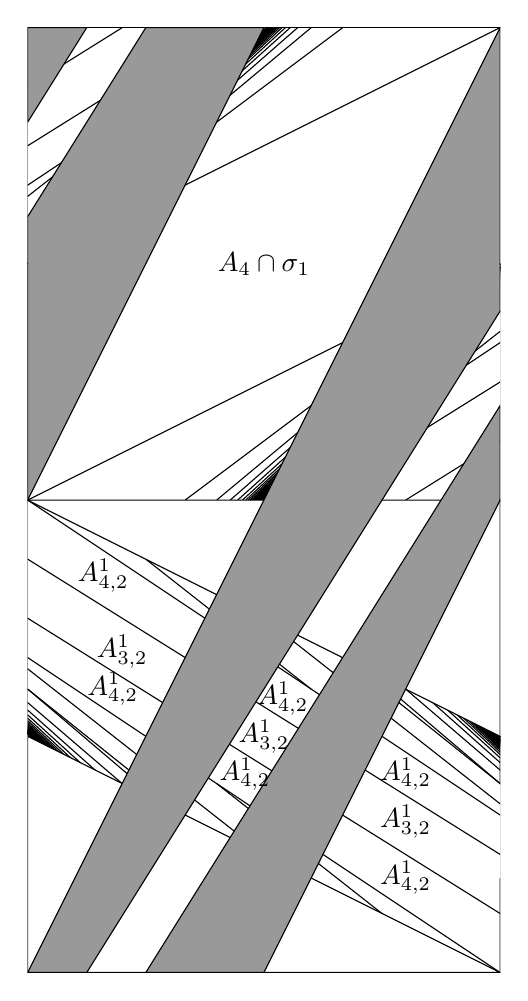
\begin{tikzpicture}[scale=1.2]
    
    \clip (0,0) rectangle (5,10);
    
    \draw (0,5) -- (10,5);
    \draw (5,10) -- (5,0);
    
    \draw (0,0) rectangle (10,10);
        
        \foreach \k in {1,...,45}{
        % Blue in R3
        \draw ({ (2*\k+2)*(7.5-7.5)/(2*\k+1)  }, { 7.5 })--({ (2*\k+2)*(10-7.5)/(2*\k+1)  }, { 10 });
        \draw ({ 5+ (2*\k+2)*(5-7.5)/(2*\k+1)  }, { 5 })--({ 5+ (2*\k+2)*(7.5-7.5)/(2*\k+1) }, { 7.5 });
        % Red in A3/A4
        \draw ({ 2.5 + (2*\k+1)*(5-5)/(2*\k)  }, { 5 })--({ 2.5 + (2*\k+1)*(10-5)/(2*\k)  }, { 10 });
        \draw ({ 12.5 + (2*\k+1)*(5-10)/(2*\k)  }, { 5 }) -- ({ 12.5 + (2*\k+1)*((30*\k+20)/(4*\k+2)-10)/(2*\k)  }, { (30*\k+20)/(4*\k+2) });
        }
        
        % Red green, n=2
        \draw (30/4,70/8) -- (4,6);
        \draw (70/8,150/16) -- (7,8);
        % Symmetries...
        \draw (15-30/4,15-70/8) -- (15-5,15-190/28);
        \draw (15-70/8,15-150/16) -- (15-7,15-8);
        % Top left corner...
        %% Red red
        \draw (2.5,10) -- (0 , 50/6);
        %% Red green
        \draw (1,9) -- (0,15-190/28);
        
        
        % Red green, n=3
        \draw (5,7)--(90/14,230/28);
        % Symmetry
        \draw (15-5,15-7)--(15-90/14,15-230/28);
        
        \filldraw[fill=white] (0,5) -- (10,10) -- (5,10) -- (0,7.5) -- (0,5);
        \filldraw[fill=white] (5,5) -- (10,7.5) -- (10,5) -- (5,5);
        
        
        % Red green, n=1
        \draw (0,150/16) -- (1,10);
        \draw (0,70/8) -- (2,10);
        \draw (10,150/16) -- (3,5);
        \draw (10,70/8) -- (4,5);
      
       % We can get other sing set lines by reflecting in x=1/2 then translating x->x-1/2
       \foreach \k in {1,...,45}{
        % Blue in R3
        \draw ({10- (2*\k+2)*(7.5-7.5)/(2*\k+1)  }, { 7.5-5 })--({10- (2*\k+2)*(10-7.5)/(2*\k+1)  }, { 10-5 });
        \draw ({ 5 - (2*\k+2)*(5-7.5)/(2*\k+1)  }, { 5-5 })--({ 5 - (2*\k+2)*(7.5-7.5)/(2*\k+1)  }, { 7.5-5 });
        % Red in A3/A4
        \draw ({ 7.5 - (2*\k+1)*(5-5)/(2*\k)  }, { 5-5 })--({ 7.5- (2*\k+1)*(10-5)/(2*\k)  }, { 10-5 });
        \draw ({ -2.5 - (2*\k+1)*(5-10)/(2*\k)  }, { 5-5 }) -- ({ -2.5 - (2*\k+1)*((30*\k+20)/(4*\k+2)-10)/(2*\k)  }, { (30*\k+20)/(4*\k+2) -5 });
        }
        
        % Red green, n=2
        \draw (10-30/4,70/8-5) -- (10-4,6-5);
        \draw (10-70/8,150/16-5) -- (10-7,8-5);
        % Symmetries...
        \draw (-5+30/4,15-70/8-5) -- (0,15-190/28-5);
        \draw (-5+70/8,15-150/16-5) -- (-5+7,15-8-5);
        % Top left corner...
        %% Red red
        \draw (10-2.5,10-5) -- (10, 50/6-5);
        %% Red green
        \draw (10-1,9-5) -- (10,15-190/28-5);
        
        
        % Red green, n=3
        \draw (10-5,7-5)--(10-90/14,230/28-5);
        % Symmetry
        \draw (0,15-7-5)--(-5+90/14,15-230/28-5);
        
        \filldraw[fill=white] (10,0) -- (0,5) -- (5,5) -- (10,2.5) -- (10,0);
        \filldraw[fill=white] (0,0) -- (5,0) -- (0,2.5) -- (0,0);
        
        
        % Red green, n=1
        \draw (10,150/16-5) -- (10-1,10-5);
        \draw (10,70/8-5) -- (10-2,10-5);
        \draw (0,150/16-5) -- (10-3,5-5);
        \draw (0,70/8-5) -- (10-4,5-5);
       
       
      \filldraw[fill=gray!80] (0,8) -- (10/8,10) -- (2.5,10) -- (0,5) -- (0,8);
      \filldraw[fill=gray!80] (0,9) -- (0,10) -- (10/16,10) -- (0,9);
      \filldraw[fill=gray!80] (0,0) -- (5,10) -- (5,7) -- (10/16,0) -- (0,0);
      \filldraw[fill=gray!80] (10/8,0) -- (2.5,0) -- (5,5) -- (5,6) -- (10/8,0) ;
      
      \filldraw[fill=gray!80] (5,2) -- (50/8,0) -- (7.5,0) -- (5,5) -- (5,2);
      \filldraw[fill=gray!80] (5,1) -- (5,0) -- (90/16,0) -- (5,1);
      \filldraw[fill=gray!80] (5,10) -- (10,0) -- (10,3) -- (90/16,10) -- (5,10);
      \filldraw[fill=gray!80] (50/8,10) -- (7.5,10) -- (10,5) -- (10,4) -- (50/8,10);
  
        \node at (2.5,7.5) {$A_4 \cap \sigma_1$};
  
      \node at (2.5,2.5) {$A_{3,2}^1$};
      \node at (1,3.4) {$A_{3,2}^1$};
      \node at (4,1.6) {$A_{3,2}^1$};
     
      \node at (2.7,2.9) {$A_{4,2}^1$};
      \node at (0.8,4.2) {$A_{4,2}^1$};
      \node at (4,2.1) {$A_{4,2}^1$};
      
      \node at (2.3,2.1) {$A_{4,2}^1$};
      \node at (0.9,3) {$A_{4,2}^1$};
      \node at (4,1) {$A_{4,2}^1$};
      
      %\draw[very thick] (190/89,215/89) -- (230/89,190/89) -- (5-190/89,5-215/89) -- (5-230/89,5-190/89) -- (190/89,215/89);
      %\node at (230/89+0.15,190/89-0.05) {$Q$};
    \end{tikzpicture}
}
\hspace{1em}
\subfigure[][]{
\label{fig:sigmaSubpartition}
     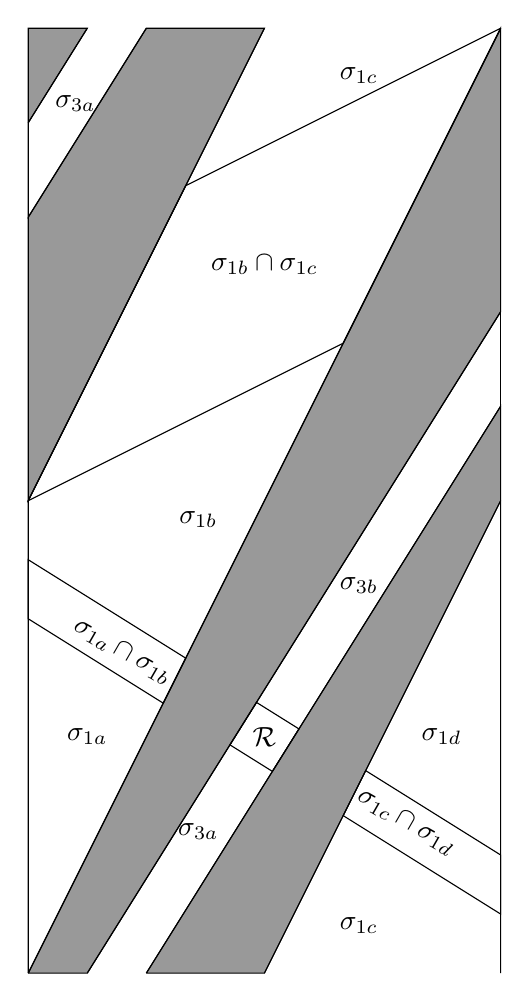
\begin{tikzpicture}[scale=1.2]
    
    \draw (0,0) -- (0,10);
     \draw (5,0) -- (5,10);

      \filldraw[fill=gray!80] (0,8) -- (10/8,10) -- (2.5,10) -- (0,5) -- (0,8);
      \filldraw[fill=gray!80] (0,9) -- (0,10) -- (10/16,10) -- (0,9);
      \filldraw[fill=gray!80] (0,0) -- (5,10) -- (5,7) -- (10/16,0) -- (0,0);
      \filldraw[fill=gray!80] (10/8,0) -- (2.5,0) -- (5,5) -- (5,6) -- (10/8,0);
 
 
    \draw (0,0) -- (0,35/8) -- (35/21,70/21) -- (0,0);
    
   \draw (5,10) -- (10/6,50/6) -- (0,5) -- (0,30/8) -- (30/21,60/21) --  (5,10);
    
   \draw (2.5,10) -- (0,5) -- (5-10/6,10-20/6) -- (5,10);
    \draw (5,0) -- (5,5-30/8) -- (5-30/21,5-60/21) --  (2.5,0);
    
    \draw (5,5) -- (5,5-35/8) -- (5-35/21,5-70/21) -- (5,5);
 
   \draw (10/8,0) -- (5-190/89,5-215/89) -- (5-230/89,5-190/89) -- (10/16,0);
    \draw (10/16,10) -- (0,9) -- (0,8) -- (10/8,10);
 
    \draw (5,7) -- (190/89,215/89) -- (230/89,190/89) -- (5,6);
 
    \node at (10/16,2.5) {$\sigma_{1a}$};
    
    \node at (1.8,4.8) {$\sigma_{1b}$};
    
    \node at (3.5,9.5) {$\sigma_{1c}$};
    \node at (3.5,0.5) {$\sigma_{1c}$};
    
    \node at (5-10/16,2.5) {$\sigma_{1d}$};
    
    \node at (0.5,9.2) {$\sigma_{3a}$};
    \node at (1.8,1.5) {$\sigma_{3a}$};
     \node at (3.5,4.1) {$\sigma_{3b}$};
    
    % \node at (2.5,2.5) {$\sigma_{3a} \cap \sigma_{3b}$};
     \node at (2.5,2.5) {$\mathcal{R}$};
     \node [rotate=-30] at (1,3.4) {$\sigma_{1a} \cap \sigma_{1b}$};
     \node [rotate=-30] at (4,1.6) {$\sigma_{1c} \cap \sigma_{1d}$};
    \node at (2.5,7.5) {$\sigma_{1b} \cap \sigma_{1c}$};
    
 
    \end{tikzpicture}
    }

   \caption{Part (a) shows the singularity curves dividing up $\sigma_1 \cup \sigma_3$ with some key partition elements labelled. The elements $A_{3,2}^1$, $A_4 \cap \sigma$ split $\sigma_1 \cup \sigma_3$ into six subsets $\sigma_{1a},\dots,\sigma_{3b}$, any two of which are either disjoint or have intersection given by $A_4 \cap \sigma$ or one of the three subsets which make up $A_{3,2}^1$, see part (b). $\mathcal{R}$ denotes the set $\sigma_{3a} \cap \sigma_{3b}$.}
    \label{fig:caseA1Partition}
\end{figure}

Let $\Gamma$ satisfy case (A1) and suppose it has non-simple intersection with $A_{4,2}^1$. Now since $\Gamma$ has simple intersection with $A_3$, observing Figure \ref{fig:singSetFT} it is clear that $\Gamma$ must traverse $A_{3,2}^1$. Restricting $\Gamma^2 = \Gamma \cap A_2$, $H\left(\Gamma^2\right) \subset H(\Gamma)$ is a line segment which has non-simple intersection with $A_4$, i.e. (C1) is satisfied with $k=1$. Assume, then, that $\Gamma$ has simple intersection with $A_{4,2}^1$ and therefore does not traverse $A_{3,2}^1$. If $\Gamma \subset \sigma_3$ then $\Gamma$ lies entirely within one of two sets $\sigma_{3a}$, $\sigma_{3b}$ (shown in Figure \ref{fig:sigmaSubpartition}) whose union is $\sigma_3$, intersection is $\mathcal{R} = A_{3,2}^1 \cap \sigma_3$. For $\Gamma \subset \sigma_1$, simple intersection with $A_3$ implies that $\Gamma$ does not traverse $A_4 \cap \sigma_1$. This, together with the two disjoint sets which make up $A_{3,2}^1 \cap \sigma_1$, implies that $\Gamma$ lies entirely within one of four subsets $\sigma_{1a},\dots,\sigma_{1d}$, shown in Figure \ref{fig:sigmaSubpartition}. The behaviour of $H_\sigma$ over the sets $\sigma_{1a}$, $\sigma_{1b}$ is shown explicitly in Figures \ref{fig:sigma1a}, \ref{fig:sigma1b}.
 
\begin{figure}
    \centering

    \begin{tikzpicture}
    \node at (0,0) {
    
    \begin{tikzpicture}[scale=4.5]
    \draw (0,1.6) -- (0,35/8) -- (35/21,70/21) -- (0.8,1.6);
    \draw[->] (1.2,2.1308) -- (1.035,2.1308);
    \node at (1.28,2.1308) {$A_{3,2}^3$}; 
    
    
\begin{scope}

    
    \clip (0,1.6) -- (0,35/8) -- (35/21,70/21) -- (0.8,1.6);
    \draw (0,5) -- (10,5);
    \draw (5,10) -- (5,0);
    
    \fill[black] (0,2.3) rectangle (0.045,2.52);
    
    \draw (0,0) rectangle (10,10);
        
        \foreach \k in {1,...,45}{
        % Blue in R3
        \draw ({ (2*\k+2)*(7.5-7.5)/(2*\k+1)  }, { 7.5 })--({ (2*\k+2)*(10-7.5)/(2*\k+1)  }, { 10 });
        \draw[blue] ({ 5+ (2*\k+2)*(5-7.5)/(2*\k+1)  }, { 5 })--({ 5+ (2*\k+2)*(7.5-7.5)/(2*\k+1) }, { 7.5 });
        % Red in A3/A4
        \draw ({ 2.5 + (2*\k+1)*(5-5)/(2*\k)  }, { 5 })--({ 2.5 + (2*\k+1)*(10-5)/(2*\k)  }, { 10 });
        \draw ({ 12.5 + (2*\k+1)*(5-10)/(2*\k)  }, { 5 }) -- ({ 12.5 + (2*\k+1)*((30*\k+20)/(4*\k+2)-10)/(2*\k)  }, { (30*\k+20)/(4*\k+2) });
        }
        
        % Red green, n=2
        \draw (30/4,70/8) -- (4,6);
        \draw (70/8,150/16) -- (7,8);
        % Symmetries...
        \draw (15-30/4,15-70/8) -- (15-5,15-190/28);
        \draw (15-70/8,15-150/16) -- (15-7,15-8);
        % Top left corner...
        %% Red red
        \draw (2.5,10) -- (0 , 50/6);
        %% Red green
        \draw (1,9) -- (0,15-190/28);
        
        
        % Red green, n=3
        \draw (5,7)--(90/14,230/28);
        % Symmetry
        \draw (15-5,15-7)--(15-90/14,15-230/28);
        
        \filldraw[fill=white] (0,5) -- (10,10) -- (5,10) -- (0,7.5) -- (0,5);
        \filldraw[fill=white] (5,5) -- (10,7.5) -- (10,5) -- (5,5);
        
        
        % Red green, n=1
        \draw (0,150/16) -- (1,10);
        \draw (0,70/8) -- (2,10);
        \draw (10,150/16) -- (3,5);
        \draw (10,70/8) -- (4,5);
      
       % We can get other sing set lines by reflecting in x=1/2 then translating x->x-1/2
       \foreach \k in {1,...,45}{
        % Blue in R3
        \draw ({10- (2*\k+2)*(7.5-7.5)/(2*\k+1)  }, { 7.5-5 })--({10- (2*\k+2)*(10-7.5)/(2*\k+1)  }, { 10-5 });
        \draw ({ 5 - (2*\k+2)*(5-7.5)/(2*\k+1)  }, { 5-5 })--({ 5 - (2*\k+2)*(7.5-7.5)/(2*\k+1)  }, { 7.5-5 });
        % Red in A3/A4
        \draw ({ 7.5 - (2*\k+1)*(5-5)/(2*\k)  }, { 5-5 })--({ 7.5- (2*\k+1)*(10-5)/(2*\k)  }, { 10-5 });
        \draw ({ -2.5 - (2*\k+1)*(5-10)/(2*\k)  }, { 5-5 }) -- ({ -2.5 - (2*\k+1)*((30*\k+20)/(4*\k+2)-10)/(2*\k)  }, { (30*\k+20)/(4*\k+2) -5 });
        }
        
        % Red green, n=2
        \draw (10-30/4,70/8-5) -- (10-4,6-5);
        \draw (10-70/8,150/16-5) -- (10-7,8-5);
        % Symmetries...
        \draw (-5+30/4,15-70/8-5) -- (0,15-190/28-5);
        \draw (-5+70/8,15-150/16-5) -- (-5+7,15-8-5);
        % Top left corner...
        %% Red red
        \draw (10-2.5,10-5) -- (10, 50/6-5);
        %% Red green
        \draw (10-1,9-5) -- (10,15-190/28-5);
        
        
        % Red green, n=3
        \draw (10-5,7-5)--(10-90/14,230/28-5);
        % Symmetry
        \draw (0,15-7-5)--(-5+90/14,15-230/28-5);
        
        \filldraw[fill=white] (10,0) -- (0,5) -- (5,5) -- (10,2.5) -- (10,0);
        \filldraw[fill=white] (0,0) -- (5,0) -- (0,2.5) -- (0,0);

        \draw (0,0) -- (5,10);
        
        % Red green, n=1
        \draw (10,150/16-5) -- (10-1,10-5);
        \draw (10,70/8-5) -- (10-2,10-5);
        \draw (0,150/16-5) -- (10-3,5-5);
        \draw (0,70/8-5) -- (10-4,5-5);

     \node at (1,3.4) {$A_{3,2}^1$};
     \node at (1.08,2.8) {$A_{4,2}^1$};
     \node at (1.08,2.48) {$A_{3,2}^2$};
     \node at (0.8,2.48) {$A_{4,2}^2$};
     \node at (0.8,2.25) {$A_{4,2}^3$};
     
     \node at (0.735,2.167) {$A_{4,2}^4$};
     
     \node at (0.4,2) {$A_1 \cap \sigma_1$};
     

\end{scope}
        \draw [red, dashed, thick] (0,2.5) -- (0,2.7) -- (0.4,2.5) -- (0.4,2.3) -- (0,2.5);
    \draw [<->, red] (0,2.27) -- (0.4,2.27);
    \draw [<->, red] (-0.03,2.5) -- (-0.03,2.7);
    \node[scale=0.7] at (-0.08,2.6) {\color{red}$\sqrt{\varepsilon}$\color{black}};
    \node[scale=0.7] at (0.2,2.3) {\color{red}$2\sqrt{\varepsilon}$\color{black}};

    \end{tikzpicture} };
    
    
    \end{tikzpicture}
    
    \caption{The singularity set of $H_\sigma$ over $\sigma_{1a}$. Unlabelled sets are given by $A_{4,2}^k$ for $k\geq 5$ which limit onto the point $(0,1/4)$ in the obvious fashion. The dashed red line is $\partial P(\varepsilon)$, useful for establishing \textbf{(KS1)} for $H_\sigma$. }
    \label{fig:sigma1a}
\end{figure}

Let $\| \cdot \|$ denote the $\| \cdot \|_\infty$ norm. Starting with $\sigma_{1a}$, $DH_\sigma$ takes values in $\mathcal{M}_{1a} = \{ M_1, M_4M_2^k, M_3M_2^l \,| \, k\in \mathbb{N}, \, l=1,2,3\}$. The unlabelled sets in Figure \ref{fig:sigma1a} are the partition elements $A_{4,2}^k$ for $k \geq 5$, limiting onto the point $(0,1/4)$ as $k\rightarrow \infty$ in the obvious fashion. We remark that any $\Gamma \subset \sigma_{1a}$ has simple intersection with all of the partition elements $A_{i,j}^k \subset \sigma_{1a}$. If $\Gamma$ is entirely contained within some partition element $A$ corresponding to $M \in \mathcal{M}_{1a}$, and is aligned with some unit vector $v\in \mathcal{C}_+$, then $\ell_v\left( H_\sigma(\Gamma) \right) = \| M v  \| \ell_v(\Gamma)$. Minimum expansion factors are straightforward to calculate. Parameterise unit vectors in $\mathcal{C}_+$ by $(v_1,1)^T$ where $1/3 \leq v_1 \leq 13/21$ and write the components of matrices $M \in \mathcal{M}$ as $\big(\begin{smallmatrix}
  a & b\\
  c & d
\end{smallmatrix}\big)$ . Then by cone invariance and the fact that vectors $(v_1,v_2)^T \in \mathcal{C}$ have norm $|v_2|$, we have that $\| M v \| = |cv_1 + d|$. This is monotone increasing in $v_1$ if $\mathrm{sgn}(c) = \mathrm{sgn}(d)$, monotone decreasing if $\mathrm{sgn}(c)\neq \mathrm{sgn}(d)$, so that $\| M v \|$ is minimal on $(1/3,1)^T$ or $(13/21,1)^T$ in these respective cases. Table \ref{tab:tab2} shows the components of matrices $M \in \mathcal{M}$ and the minimum expansion factors $K_+(M)$ which follow.

% \begin{table}[ht]
%     \centering
%     \begin{tabular}{c|c|c}
%         $M$ & Components & $K_+(M)$ \\ \hline
% $M_1$ & $ \left(\begin{matrix}1 & 2\\2 & 5\end{matrix}\right) $ & \( \displaystyle  \frac{17}{3} \)  \\
% $M_4$ & $ \left(\begin{matrix}1 & -2\\-2 & 5\end{matrix}\right) $ & \( \displaystyle  \frac{79}{21} \)  \\
% $M_1M_2^n$ & $(-1)^n \left(\begin{matrix}2 n + 1 & 2 n + 2\\6 n + 2 & 6 n + 5\end{matrix}\right) $ & \( \displaystyle  8 n + \frac{17}{3} \)  \\
% $M_1M_3^n$ & $(-1)^n \left(\begin{matrix}1 - 6 n & 6 n + 2\\2 - 14 n & 14 n + 5\end{matrix}\right) $ & \( \displaystyle  \frac{16 n}{3} + \frac{131}{21} \)  \\
% $M_2M_3^n$ & $(-1)^n \left(\begin{matrix}1 - 6 n & 6 n + 2\\10 n - 2 & - 10 n - 3\end{matrix}\right) $ & \( \displaystyle  \frac{80 n}{21} + \frac{89}{21} \)  \\
% $M_3M_2^n$ & $(-1)^n \left(\begin{matrix}1 - 6 n & - 6 n - 2\\2 - 10 n & - 10 n - 3\end{matrix}\right) $ & \( \displaystyle  \frac{40 n}{3} + \frac{7}{3} \)  \\
% $M_4M_2^n$ & $(-1)^n \left(\begin{matrix}1 - 6 n & - 6 n - 2\\14 n - 2 & 14 n + 5\end{matrix}\right) $ & \( \displaystyle  \frac{56 n}{3} + \frac{13}{3} \)  \\
% $M_4M_3^n$ & $(-1)^n \left(\begin{matrix}2 n + 1 & - 2 n - 2\\- 6 n - 2 & 6 n + 5\end{matrix}\right) $ & \( \displaystyle  \frac{16 n}{7} + \frac{79}{21} \)  \\
%     \end{tabular}
%     \caption{Minimum expansion factors $K_+(M) = \inf_{v\in \mathcal{C}_+}\| M v \| / \| v \|$ for each $M \in \mathcal{M}$ over the cone $\mathcal{C}_+$.}
%     \label{tab:tab2}
% \end{table}

\begin{table}[ht]
    \centering
    \begin{tabular}{c|c|c|c}
        $M$ & Components & $K_+(M)$ & $K_-(M)$ \\ \hline
$M_1$ & $\left(\begin{matrix}1 & 2\\2 & 5\end{matrix}\right) $ & \( \displaystyle  \frac{17}{3} \) & \( \displaystyle  \frac{79}{21} \)  \\
$M_4$ & $ \left(\begin{matrix}1 & -2\\-2 & 5\end{matrix}\right) $ & \( \displaystyle  \frac{79}{21} \) & \( \displaystyle  \frac{17}{3} \)  \\
$M_1M_2^n$ & $(-1)^n \left(\begin{matrix}2 n + 1 & 2 n + 2\\6 n + 2 & 6 n + 5\end{matrix}\right) $ & \( \displaystyle  8 n + \frac{17}{3} \) & \( \displaystyle  \frac{16 n}{7} + \frac{79}{21} \)  \\
$M_1M_3^n$ & $(-1)^n \left(\begin{matrix}1 - 6 n & 6 n + 2\\2 - 14 n & 14 n + 5\end{matrix}\right) $ & \( \displaystyle  \frac{16 n}{3} + \frac{131}{21} \) & \( \displaystyle  \frac{56 n}{3} + \frac{13}{3} \)  \\
$M_2M_3^n$ & $(-1)^n \left(\begin{matrix}1 - 6 n & 6 n + 2\\10 n - 2 & - 10 n - 3\end{matrix}\right) $ & \( \displaystyle  \frac{80 n}{21} + \frac{89}{21} \) & \( \displaystyle  \frac{40 n}{3} + \frac{7}{3} \)  \\
$M_3M_2^n$ & $(-1)^n \left(\begin{matrix}1 - 6 n & - 6 n - 2\\2 - 10 n & - 10 n - 3\end{matrix}\right) $ & \( \displaystyle  \frac{40 n}{3} + \frac{7}{3} \) & \( \displaystyle  \frac{80 n}{21} + \frac{89}{21} \)  \\
$M_4M_2^n$ & $(-1)^n \left(\begin{matrix}1 - 6 n & - 6 n - 2\\14 n - 2 & 14 n + 5\end{matrix}\right) $ & \( \displaystyle  \frac{56 n}{3} + \frac{13}{3} \) & \( \displaystyle  \frac{16 n}{3} + \frac{131}{21} \)  \\
$M_4M_3^n$ & $(-1)^n \left(\begin{matrix}2 n + 1 & - 2 n - 2\\- 6 n - 2 & 6 n + 5\end{matrix}\right) $ & \( \displaystyle  \frac{16 n}{7} + \frac{79}{21} \) & \( \displaystyle  8 n + \frac{17}{3} \)  \\
    \end{tabular}
    \caption{Minimum expansion factors $K_\pm(M) = \inf_{v\in \mathcal{C}_\pm}\| M v \| / \| v \|$ for each $M \in \mathcal{M}$ over the cones $\mathcal{C}_\pm$.}
    \label{tab:tab2}
\end{table}


If $\Gamma$ intersects $A_{4,2}^4$ and $A_{3,2}^3$ (traversing $A_{4,2}^3$) then $H^{3}\left(\Gamma \cap A_{4,2}^3\right)$ is a line segment in $A_2' \cap A_4$, connecting the $A_3,A_4$ boundary to the $A_2,A_4$ boundary. Noting that $A_2' \cap A_4$ is made up of two quadrilaterals, see Figure \ref{fig:firstPartitions}, there are two possible ways this can occur. Firstly, it can connect points $(x,1)$ to $(2y -1,y)$ with $ 1/2 \leq x\leq 3/4$. Its image under $F$ then connects $(x,1)$ to $(1,y)$ so that then, shearing vertically by $G$, its image under $H$ connects $(x,2-2x)$ to $(1,y)$, passing through $y=0$. Since $x \leq 3/4$, we have $2-2x \geq 1/2$ so that $H^4\left(\Gamma \cap A_{4,2}^3\right)$ must have non-simple intersection with $A_2$. The second case, where $H^3\left(\Gamma \cap A_{4,2}^3\right)$ connects points $(x,1/2)$ and $(2y-1/2,y)$, is similar so that (C1) is satisfied.

Assume, then, that $\Gamma$ does not traverse $A_{4,2}^3$. Two possible cases follow; either $\Gamma$ lies entirely below the upper boundary of $A_{4,2}^3$, or $\Gamma$ lies entirely above the lower boundary of $A_{4,2}^3$. In the first case let $\Gamma_1 = \Gamma \cap A_1$. If $K_+(M_1) \, \ell_v(\Gamma_1) > \ell_v(\Gamma)$, then we may take $\Lambda = H(\Gamma_1) \subset H_\sigma(\Gamma)$ to satisfy (C2). Taking $K_+(M_1) = 17/3$ from Table \ref{tab:tab2}, this holds provided that $\ell_v(\Gamma_1)/\ell_v(\Gamma) > 3/17$. Noting that $\Gamma \subset A_1 \cup A_2$, if the above inequality does not hold, then the proportion of $\Gamma$ in $A_2$ satisfies $\ell_v(\Gamma_2)/\ell_v(\Gamma) > 14/17$. Observing Figure \ref{fig:sigma1a}, $\Gamma_2$ intersects some collection of sets $A_{4,2}^k$, indexed by a consecutive subset $\{ k_0, k_0+1, ...\}\subset \mathbb{N}$ with $k_0 \geq 3$. Assume that $\Gamma_2$ intersects just two of these sets $\Gamma_2 = \Gamma_{k_0} \cup \Gamma_{k_0+1}$. As seen in \cite{myers_hill_exponential_2022}, if 
\[\frac{1}{K_+\left(M_4M_2^{k_0}\right)} + \frac{1}{K_+\left(M_4M_2^{k_0+1}\right)} < 1 \]
then at least one of $\Gamma_k = \Gamma_{k_0}$, $\Gamma_{k_0+1}$ satisfies $\ell_v\left(H^{k+1}(\Gamma_k)\right) > \ell_v(\Gamma_2)$ and by extension if 
\[\frac{1}{K_+\left(M_4M_2^{k_0}\right)} + \frac{1}{K_+\left(M_4M_2^{k_0+1}\right)} < \frac{1}{\alpha} \]
then $\ell_v\left(H^{k+1}(\Gamma_k)\right) > \alpha \ell_v(\Gamma_2)$. Now noting that $K_+\left(M_4M_2^k\right)$ is monotonic increasing in $k$ we have
\[\sum_{k=k_0}^{k_0+1} \frac{1}{K_+\left(M_4M_2^k\right)} \leq \sum_{k=3}^4 \frac{1}{K_+\left(M_4M_2^k\right)} = \frac{3}{181} + \frac{3}{237} < \frac{14}{17} \]
so that, together with $\ell_v(\Gamma_2)/\ell_v(\Gamma) > 14/17$, for some $k$ condition (C2) follows by taking $\Lambda = H^{k+1}\left(\Gamma \cap A_{4,2}^k\right)$. The case where $\Gamma$ intersects just one of the $A_{4,2}^k$ follows as a trivial consequence.

Suppose $\Gamma \subset \sigma_{1a}$ violates the lemma, by the above we have that $\Gamma$ intersects three or more of the $A_{4,2}^k$, which by the geometry of the partition (see Figure \ref{fig:sigma1a}) implies
\begin{enumerate}[label={($\dagger$)}]
    \item $\Gamma$ traverses $A_{4,2}^k$ for some $k \geq 4$, connecting the lines $\mathcal{L}_k:$ $y=\frac{k+1-4kx}{4k+2}$ and $\mathcal{L}_{k-1}:$ $y=\frac{k-4(k-1)x}{4k-2}$.
\end{enumerate}
We will show that this leads to a contradiction through an inductive argument. If $\Gamma$ intersects $A_{4,2}^3$, it must traverse $A_{4,2}^4$. Let $y_k = (k+1)/(4k+2)$ be the sequence of points where $\mathcal{L}_k$ meets $x=0$. Since the gradients of $\mathcal{L}_k$ are monotone decreasing in $k$, a lower bound $h_4 \leq \ell_v\left(\Gamma \cap A_{4,2}^4\right)$ is given by $y_4'-y_4$ where $(x_4',y_4')$ is the intersection of the lines $y=y_4+\varphi x$ and $\mathcal{L}_3: \, y= (4-12x)/14$. Specifically
\begin{equation}
    \label{eq:h4}
    h_4 = \frac{191}{675} - \frac{5}{18} = \frac{7}{1350}.
\end{equation}
As before let $\Gamma_2 = \Gamma \cap A_2$. Observing Figure \ref{fig:sigma1a}, since $\mathcal{L}_3$ meets the boundary of $A_1$ and $A_2$ at the point $(1/10,1/5)$, the height of $\Gamma_2$ is bounded by $\ell_v(\Gamma_2) \leq L_3 = y_2 - 1/5 = 1/10$. Letting $\Lambda = H^5\left(\Gamma \cap A_{4,2}^4\right)$, we have that
\[ \ell_v(\Lambda) \geq K_+\left(M_4M_2^4\right)\, h_4 = \frac{56(4) + 13}{3} \frac{7}{1350} = \frac{553}{1350} \approx 0.4096 \]
and
$\ell_v(\Gamma) < (17/14) \, \ell_v(\Gamma_2) \leq 17/140 \approx 0.1214$, so that (C2) is satisfied. For the inductive step, assume that $\Gamma$ traverses $A_{4,2}^k$, but does not traverse $A_{4,2}^{k-1}$. Using the same method as before we calculate
\begin{equation}
    \label{eq:hk}
    h_k = \frac{21}{2\left(2k+1\right)\left(68k-47\right)}
\end{equation}
and
\begin{equation}
    \label{eq:Lk-1}
    L_{k-1} = \frac{k-1}{4k-6} - \frac{k-1}{4k-2} \frac{\left(k-1\right)}{\left(2k-3\right)\left(2k-1\right)}.
\end{equation}
Then (C2) is satisfied with $\Lambda = H^{k+1}\left(\Gamma \cap A_{4,2}^k\right)$ provided that $K_+\left(M_4M_2^k\right) \, h_k > (17/14) L_{k-1}$, i.e.
\begin{equation}
    \label{eq:sigma1aInductiveStep}
    \frac{56k+13}{3} \frac{21}{2\left(2k+1\right)\left(68k-47\right)} - \frac{17}{14} \frac{\left(k-1\right)}{\left(2k-3\right)\left(2k-1\right)} > 0,
\end{equation}
which holds for all $k>4$ as required. It follows by induction that if $\Gamma$ violates the lemma it must not traverse any $A_{4,2}^k$ for $k\geq 3$, contradicting ($\dagger$), so that the lemma must hold when $\Gamma \subset \sigma_{1a}$ lies entirely below the upper boundary of $A_{4,2}^3$. The case where $\Gamma\subset \sigma_{1a}$ lies entirely above the lower boundary of $A_{4,2}^3$ is more straightforward, with (C2) following from the inequality
\begin{equation}
    \label{eq:sigma1aSimple}
    \sum_{k=1}^3 \frac{1}{K_+\left( M_3M_2^k\right)} +  \frac{1}{K_+\left(M_4M_2^k\right)} = \sum_{k=1}^3 \frac{3}{56k+13} + \frac{3}{40k+7} \approx 0.206 < 1.
\end{equation}
The lemma holds, then, for general $\Gamma \subset \sigma_{1a}$.


\begin{figure}
    \centering
    \begin{tikzpicture}
    \node at (0,0) {
        \begin{tikzpicture}[scale=3]
    
    \draw[->] (2.1,3.965) -- (1.88,3.965);
    \node at (2.2,3.965) {$A_{3,2}^2$};
        
    \draw[<->] (70/19+0.05,5) -- (70/19+0.05,140/19);
    \node at (3.9,235/38) {$L_0$};
    
    \draw  (1,7) -- (0,5) -- (0,30/8) -- (30/21,60/21) --  (3.75,7.5);
    \clip (0,30/8) -- (30/21,60/21) -- (3.75,7.5) -- (1,7) -- (0,5) -- (0,30/8);
    \draw (0,5) -- (10,5);
    \draw (5,10) -- (5,0);
    
    \fill[black] (2.48,5) rectangle (2.54,5.04);
    
    \draw (0,0) rectangle (10,10);
        
        \foreach \k in {1,...,45}{
        % Blue in R3
        \draw ({ (2*\k+2)*(7.5-7.5)/(2*\k+1)  }, { 7.5 })--({ (2*\k+2)*(10-7.5)/(2*\k+1)  }, { 10 });
        \draw ({ 5+ (2*\k+2)*(5-7.5)/(2*\k+1)  }, { 5 })--({ 5+ (2*\k+2)*(7.5-7.5)/(2*\k+1) }, { 7.5 });
        % Red in A3/A4
        \draw ({ 2.5 + (2*\k+1)*(5-5)/(2*\k)  }, { 5 })--({ 2.5 + (2*\k+1)*(10-5)/(2*\k)  }, { 10 });
        \draw ({ 12.5 + (2*\k+1)*(5-10)/(2*\k)  }, { 5 }) -- ({ 12.5 + (2*\k+1)*((30*\k+20)/(4*\k+2)-10)/(2*\k)  }, { (30*\k+20)/(4*\k+2) });
        }
        
        % Red green, n=2
        \draw (30/4,70/8) -- (4,6);
        \draw (70/8,150/16) -- (7,8);
        % Symmetries...
        \draw (15-30/4,15-70/8) -- (15-5,15-190/28);
        \draw (15-70/8,15-150/16) -- (15-7,15-8);
        % Top left corner...
        %% Red red
        \draw (2.5,10) -- (0 , 50/6);
        %% Red green
        \draw (1,9) -- (0,15-190/28);
        
        
        % Red green, n=3
        \draw (5,7)--(90/14,230/28);
        % Symmetry
        \draw (15-5,15-7)--(15-90/14,15-230/28);
        
        \filldraw[fill=white] (0,5) -- (10,10) -- (5,10) -- (0,7.5) -- (0,5);
        %\filldraw[fill=white] (5,5) -- (10,7.5) -- (10,5) -- (5,5);
        
        
        % Red green, n=1
        \draw (0,150/16) -- (1,10);
        \draw (0,70/8) -- (2,10);
        \draw (10,150/16) -- (3,5);
        \draw (10,70/8) -- (4,5);
      
       % We can get other sing set lines by reflecting in x=1/2 then translating x->x-1/2
       \foreach \k in {1,...,45}{
        % Blue in R3
        \draw ({10- (2*\k+2)*(7.5-7.5)/(2*\k+1)  }, { 7.5-5 })--({10- (2*\k+2)*(10-7.5)/(2*\k+1)  }, { 10-5 });
        \draw ({ 5 - (2*\k+2)*(5-7.5)/(2*\k+1)  }, { 5-5 })--({ 5 - (2*\k+2)*(7.5-7.5)/(2*\k+1)  }, { 7.5-5 });
        % Red in A3/A4
        \draw ({ 7.5 - (2*\k+1)*(5-5)/(2*\k)  }, { 5-5 })--({ 7.5- (2*\k+1)*(10-5)/(2*\k)  }, { 10-5 });
        \draw[red] ({ -2.5 - (2*\k+1)*(5-10)/(2*\k)  }, { 5-5 }) -- ({ -2.5 - (2*\k+1)*((30*\k+20)/(4*\k+2)-10)/(2*\k)  }, { (30*\k+20)/(4*\k+2) -5 });
        }
        
        % Red green, n=2
        \draw (10-30/4,70/8-5) -- (10-4,6-5);
        \draw (10-70/8,150/16-5) -- (10-7,8-5);
        % Symmetries...
        \draw (-5+30/4,15-70/8-5) -- (0,15-190/28-5);
        \draw (-5+70/8,15-150/16-5) -- (-5+7,15-8-5);
        % Top left corner...
        %% Red red
        \draw (10-2.5,10-5) -- (10, 50/6-5);
        %% Red green
        \draw (10-1,9-5) -- (10,15-190/28-5);
        
        
        % Red green, n=3
        \draw (10-5,7-5)--(10-90/14,230/28-5);
        % Symmetry
        \draw (0,15-7-5)--(-5+90/14,15-230/28-5);
        
        \filldraw[fill=white] (10,0) -- (0,5) -- (5,5) -- (10,2.5) -- (10,0);
        \filldraw[fill=white] (0,0) -- (5,0) -- (0,2.5) -- (0,0);

        \draw (0,0) -- (5,10);
        \draw (0,5) -- (2.5,10);
        
        % Red green, n=1
        \draw (10,150/16-5) -- (10-1,10-5);
        \draw (10,70/8-5) -- (10-2,10-5);
        \draw (0,150/16-5) -- (10-3,5-5);
        \draw (0,70/8-5) -- (10-4,5-5);

    \node at (1.199,4.296) {$A_{4,2}^2$};
      
    \node at (1.199,3.9) {$A_{4,2}^1$};
    
    \node at (1,3.4) {$A_{3,2}^1$};
    
    \node at (1.6,4.7) {$A_1 \cap \sigma_1$};
    
    \draw[dashed] (0,70/12) -- (10,10);  
     
    \node at (1.6,5.4) {$A_{4,3}^1$};
     \node at (1.6,6.1) {$A_4 \cap \sigma_1$};
      
         \node[scale=1.5] at (2,6.78) {$\mathcal{P}$}; 
      
    \end{tikzpicture}};
         
  
    \end{tikzpicture}     
         
      \caption{The singularity set of $H_\sigma$ over the lower part of $\sigma_{1b}$ with the top portion of $A_4 \cap \sigma_1$ omitted. Unlabelled sets are given by $A_{4,3}^k$ for $k\geq 2$ which limit onto the point $(1/4,1/2)$ in the obvious fashion. The segment $\mathcal{P}$ is the preimage under $H$ of the segment joining $(1/2,3/4)$ to $(1,1)$ in $S_4$. The length $L_0$ denotes maximum height of any segment in $\sigma_{1b}$ bounded by $\mathcal{P}$ and $y=1/2$.}
    \label{fig:sigma1b}
\end{figure}

Moving onto the case $\Gamma \subset \sigma_{1b}$, write its intersections with the lower and upper regions $y\leq 1/2$ and $y \geq 1/2$ as $\Gamma_L$ and $\Gamma_U$ respectively. Observing Figure \ref{fig:sigma1b}, $\Gamma_L$ can intersect up to 5 partition elements from $\mathcal{A}_L = \{ A_{3,2}^1, \dots, A_1 \cap \sigma \}$, on which $DH_\sigma$ takes a value in $\mathcal{M}_L = \{ M_1, M_3M_2^k, M_4M_2^k \, | \, k=1,2 \}$.
Let
\[ \alpha = \sum_{M \in \mathcal{M}_L} {\frac{1}{K_+(M)}} = \frac{3}{17}+ \sum_{k=1}^{2}\left(\frac{3}{40k+7}+\ \frac{3}{56k+13}\right) \approx 0.342. \]
Dividing through by $\alpha$, for any subset $\mathcal{N} \subset \mathcal{M}_L$ (including $\varnothing$ and $\mathcal{M}_L$) we have
\[ \sum_{M \in \mathcal{N}} {\frac{1}{\alpha K_+(M)}} \leq 1. \]
Hence we may always expand from some $A \in \mathcal{A}_L$, taking $\Lambda = H_\sigma(\Gamma \cap A)$, which by the above inequality satisfies $\alpha \ell_v(\Lambda) \geq \ell_v(\Gamma_L)$. Hence (C2) is satisfied when $\ell_v(\Gamma_L) > \alpha \ell_v(\Gamma)$. It remains to show the case $\ell_v(\Gamma_L) \leq \alpha \ell_v(\Gamma)$, i.e.
\begin{equation}
    \label{eq:GammaUproportion}
    \ell_v(\Gamma_U) \geq (1-\alpha) \ell_v(\Gamma).
\end{equation}
Observing Figure \ref{fig:sigma1b}, the set of partition elements which $\Gamma_U$ can intersect is given by $\mathcal{A}_U = \{ A_4 \cap \sigma_1, A_{4,3}^k \, | \, k \geq 1 \}$, so $\mathcal{M}_U = \{ M_4, M_4M_3^k \, | \, k \geq 1 \}$. Note that any two element subset $\mathcal{N} \subset \mathcal{M}_U$ satisfies
\begin{equation}
    \begin{split}
        \sum_{M \in \mathcal{N}} \frac{1}{ K_+(M)} & \leq \frac{1}{K_+(M_4)} + \frac{1}{K_+(M_4M_3)} \\
        & = \frac{21}{79} + \frac{21}{127} = \beta \approx 0.431
    \end{split}
\end{equation}
and $\alpha + \beta <1$. It follows that if $\Gamma_U$ intersects two or fewer of the elements of $\mathcal{A}_U$, we can guarantee (C2) by the standard method, summing the reciprocals of expansion factors. Assume, then, that $\Gamma_U$ intersects three or more elements from $\mathcal{A}_U$. It follows that
\begin{enumerate}[label={($\ddag$)}]
    \item $\Gamma_U$ traverses $A_{4,3}^k$ for some $k \geq 1$, connecting the lines $\mathcal{L}_k:$ $y=\frac{(4k+2)x + k+2}{4k+4}$ and $\mathcal{L}_{k-1}:$ $y=\frac{(4k-2)x +k+1}{4k}$.
\end{enumerate}
We now follow a similar inductive argument to before, assuming that $\Gamma$ violates the lemma and aiming to contradict ($\ddag$). Let $(x_k,y_k) = \left( \frac{k+2}{4k+6}, \frac{k+2}{2k+3} \right)$ denote the intersections of the lines $\mathcal{L}_k$ with the boundary $y=2x$ of $\sigma$. Assume $\Gamma$ traverses $A_{4,3}^k$, write its restriction to this set as $\Gamma^k$. Since the gradients of the $\mathcal{L}_k$ are monotonic increasing in $k$ and vectors in $\mathcal{C}_+$ have gradients bounded above by 3, A lower bound on $\ell_v(\Gamma_k)$ is given $h_k = y_k'-y_k$, where $(x_k',y_k')$ is the intersection of the line $y-y_k = 3(x-x_k)$ and $\mathcal{L}_{k-1}$, in particular
\begin{equation}
    \label{eq:sigma1bhk}
    h_k = \frac{8k^2+18k+7}{16k^2+28k+6} - \frac{k+2}{2k+3} = \frac{3}{16k^2+28k+6}.
\end{equation}
For the base case suppose that $\Gamma_U$ traverses $A_{4,3}^1$. Let $(x_U,y_U)$ be the intersection with $y=1/2 + x/2$, the boundary between $A_{4,3}^1$ and $A_4 \cap \sigma_1$. Note that this point maps to $(1,y_U)$ under $H$ with $y_U<2/3$. Figure \ref{fig:sigma1b} shows the preimage $\mathcal{P}$ in $A_4 \cap \sigma_1$ of the segment joining $(1/2,3/4)$ to $(1,1)$ between $A_3$ and $A_4$. Specifically $\mathcal{P}$ lies on the line $y = 7/12 + 5x/12$ and $H(\mathcal{P})$ lies on $y = 1/2 + x/2$. If $\Gamma$ intersects $\mathcal{P}$, then $H(\Gamma)$ connects $(1,y_U)$ to a point on the segment joining $(1/2,3/4)$ to $(1,1)$. Since $y_U< 3/4$, it follows that $H(\Gamma)$ traverses $A_3$, making non-simple intersection with $A_4$, so that (C1) is satisfied. Assume, then, that $\Gamma_U$ does not intersect $\mathcal{P}$. This gives an upper bound $\ell_v(\Gamma_U) \leq y_0 - 1/2 =: L_0$, where $(x_0,y_0) = (7/19,14/19)$ is the intersection of $\mathcal{P}$ with the boundary of $\sigma_{1}$ on $y=2x$ (see Figure \ref{fig:sigma1b}). Noting (\ref{eq:GammaUproportion}), (C2) follows with $\Lambda = H^2\left(\Gamma^1\right)$ if the inequality $K_+(M_4M_3) h_1 > L_0/(1-\alpha)$ is satisfied. Indeed
\[ \left(\frac{16}{7} + \frac{79}{21}\right) \frac{3}{16+28+6} - \frac{9}{38(1-\alpha) } \approx 0.00277 > 0 \]
so that the base step of the induction holds. The inductive step is roughly analogous, reducing to checking the inequality 
\begin{equation}
\label{eq:sigma1bInduction}
    K_+\left(M_4M_3^k\right) h_k - \frac{L_{k-1}}{1-\alpha} >0,
\end{equation} where $L_{k-1} = y_{k-2} - 1/2$ is the height of the partition element $A_{4,3}^{k-1}$. One can verify that this inequality holds (the function is monotonic decreasing in $k\geq 2$ with limit $0$ as $k \rightarrow \infty$), establishing the lemma for $\Gamma \subset \sigma_{1b}$.

\begin{figure}
    \centering

    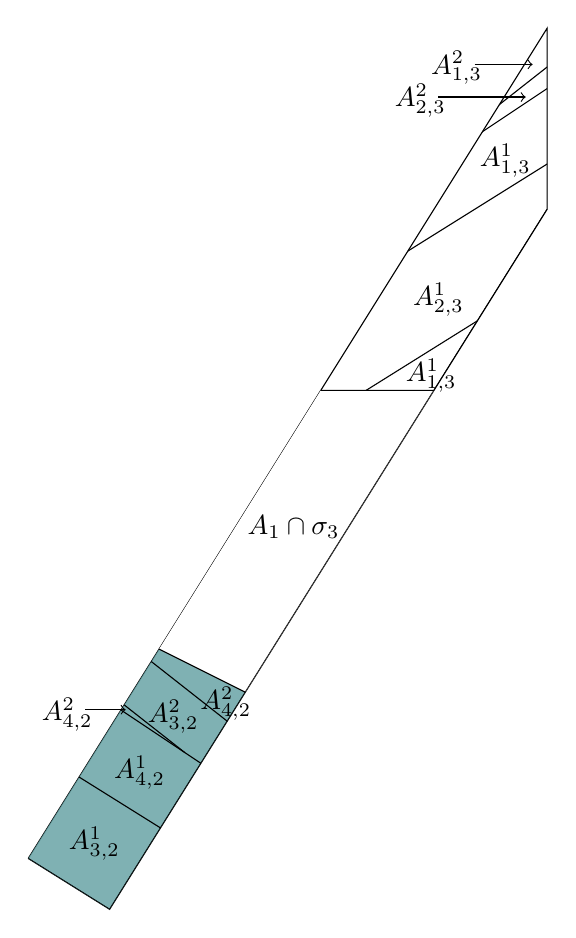
\begin{tikzpicture}[scale=2.3]
    \draw (190/89,215/89) -- (230/89,190/89) --  (5,6) -- (5,7) -- (190/89,215/89);
    
    \definecolor{tomato}{RGB}{255, 99, 71}
    \definecolor{teal}{RGB}{95, 158, 160} 
    
    \fill[fill=teal,opacity=0.8] (190/89, 430/178) -- (230/89,190/89) -- (10/3,10/3) -- (20/7,50/14) -- (190/89, 430/178);
    
    \node at (3.226,3.271) {$A_{4,2}^2$};
    
    \node at (4.36,5.08) {$A_{1,3}^1$};
    \node at (2.75,2.89) {$A_{4,2}^1$};
    
    \draw[->] (2.45,3.237) -- (2.673,3.237);
    \node at (2.35,3.21) {$A_{4,2}^2$};
    
    
    \draw[->] (4.4,6.62) -- (4.882,6.62);
    \node at (4.3,6.6) {$A_{2,3}^2$};
    
    \draw[->] (4.6,6.8) -- (4.92,6.8);
    \node at (4.5,6.78) {$A_{1,3}^2$};
    
    \clip (190/89,215/89) -- (230/89,190/89) --  (5,6) -- (5,7) -- (190/89,215/89);
    \draw (0,5) -- (10,5);
    \draw (5,10) -- (5,0);
    
    \draw (0,0) rectangle (10,10);
        
        \foreach \k in {1,...,45}{
        % Blue in R3
        \draw ({ (2*\k+2)*(7.5-7.5)/(2*\k+1)  }, { 7.5 })--({ (2*\k+2)*(10-7.5)/(2*\k+1)  }, { 10 });
        \draw[blue] ({ 5+ (2*\k+2)*(5-7.5)/(2*\k+1)  }, { 5 })--({ 5+ (2*\k+2)*(7.5-7.5)/(2*\k+1) }, { 7.5 });
        % Red in A3/A4
        \draw ({ 2.5 + (2*\k+1)*(5-5)/(2*\k)  }, { 5 })--({ 2.5 + (2*\k+1)*(10-5)/(2*\k)  }, { 10 });
        \draw ({ 12.5 + (2*\k+1)*(5-10)/(2*\k)  }, { 5 }) -- ({ 12.5 + (2*\k+1)*((30*\k+20)/(4*\k+2)-10)/(2*\k)  }, { (30*\k+20)/(4*\k+2) });
        }
        
        % Red green, n=2
        \draw (30/4,70/8) -- (4,6);
        \draw (70/8,150/16) -- (7,8);
        % Symmetries...
        \draw (15-30/4,15-70/8) -- (15-5,15-190/28);
        \draw (15-70/8,15-150/16) -- (15-7,15-8);
        % Top left corner...
        %% Red red
        \draw (2.5,10) -- (0 , 50/6);
        %% Red green
        \draw (1,9) -- (0,15-190/28);
        
        
        % Red green, n=3
        \draw (5,7)--(90/14,230/28);
        % Symmetry
        \draw (15-5,15-7)--(15-90/14,15-230/28);
        
        \filldraw[fill=white] (0,5) -- (10,10) -- (5,10) -- (0,7.5) -- (0,5);
        \filldraw[fill=white] (5,5) -- (10,7.5) -- (10,5) -- (5,5);
        
        
        % Red green, n=1
        \draw (0,150/16) -- (1,10);
        \draw (0,70/8) -- (2,10);
        \draw (10,150/16) -- (3,5);
        \draw (10,70/8) -- (4,5);
      
       % We can get other sing set lines by reflecting in x=1/2 then translating x->x-1/2
       \foreach \k in {1,...,45}{
        % Blue in R3
        \draw ({10- (2*\k+2)*(7.5-7.5)/(2*\k+1)  }, { 7.5-5 })--({10- (2*\k+2)*(10-7.5)/(2*\k+1)  }, { 10-5 });
        \draw ({ 5 - (2*\k+2)*(5-7.5)/(2*\k+1)  }, { 5-5 })--({ 5 - (2*\k+2)*(7.5-7.5)/(2*\k+1)  }, { 7.5-5 });
        % Red in A3/A4
        \draw ({ 7.5 - (2*\k+1)*(5-5)/(2*\k)  }, { 5-5 })--({ 7.5- (2*\k+1)*(10-5)/(2*\k)  }, { 10-5 });
        \draw[red] ({ -2.5 - (2*\k+1)*(5-10)/(2*\k)  }, { 5-5 }) -- ({ -2.5 - (2*\k+1)*((30*\k+20)/(4*\k+2)-10)/(2*\k)  }, { (30*\k+20)/(4*\k+2) -5 });
        }
        
        % Red green, n=2
        \draw (10-30/4,70/8-5) -- (10-4,6-5);
        \draw (10-70/8,150/16-5) -- (10-7,8-5);
        % Symmetries...
        \draw (-5+30/4,15-70/8-5) -- (0,15-190/28-5);
        \draw (-5+70/8,15-150/16-5) -- (-5+7,15-8-5);
        % Top left corner...
        %% Red red
        \draw (10-2.5,10-5) -- (10, 50/6-5);
        %% Red green
        \draw (10-1,9-5) -- (10,15-190/28-5);
        
        
        % Red green, n=3
        \draw (10-5,7-5)--(10-90/14,230/28-5);
        % Symmetry
        \draw (0,15-7-5)--(-5+90/14,15-230/28-5);
        
        \filldraw[fill=white] (10,0) -- (0,5) -- (5,5) -- (10,2.5) -- (10,0);
        \filldraw[fill=white] (0,0) -- (5,0) -- (0,2.5) -- (0,0);
        \draw (5,6) -- (10/8,0);
        
        % Red green, n=1
        \draw (10,150/16-5) -- (10-1,10-5);
        \draw (10,70/8-5) -- (10-2,10-5);
        \draw (0,150/16-5) -- (10-3,5-5);
        \draw (0,70/8-5) -- (10-4,5-5);

        \node at (2.5,2.5) {$A_{3,2}^1$};

        \node at (2.935,3.2) {$A_{3,2}^2$};

        \node at (3.6,4.245) {$A_1 \cap \sigma_3$};

        \node at (4.4,5.5) {$A_{2,3}^1$};
        \node at (4.769,6.27) {$A_{1,3}^1$};
      
    \end{tikzpicture}
    
      \caption{Behaviour of $H_\sigma$ over $\sigma_{3b} \setminus \varsigma_3$ and $H_\sigma^2$ over $\varsigma_3$, shaded in blue.}
    \label{fig:sigma3b}
\end{figure}
    
Next consider $\Gamma \subset \sigma_{3b}$, shown in Figure \ref{fig:sigma3b}. Note that outside of $\varsigma_3$ (shaded in blue) the Jacobian $DH_\sigma$ is some matrix from $\mathcal{M}$, but over $\varsigma_3$ we have $DH_\sigma = M_2 \notin \mathcal{M}$. Therefore if we are to expand from some subset of $\Gamma \cap \varsigma_3$, to ensure that $\Lambda$ satisfies one of (A1-2) we must map forwards using $H_\sigma^2$, whose Jacobian is always a matrix from $\mathcal{M}$ (analogous to the escape behaviour shown for $A_3$, shown in Figure \ref{fig:escapeBehaviour}). The relevant subset of matrices, then, is $\mathcal{M}_{3b} = \{M_1, M_1M_3^k, M_2M_3^k, M_3M_2^k, M_4M_2^k \,| \, k=1,2 \}$. Noting that $\Gamma$ can have non-simple intersection with the sets $A_{4,2}^2$ and $A_{1,3}^1$, the relevant inequality to verify is
\[ \left (\sum_{M \in \mathcal{M}_{3b}} \frac{1}{K_+(M)} \right ) + \frac{1}{K_+(M_1M_3)} + \frac{1}{K_+\left(M_4M_2^2\right)} < 1. \]
Indeed, the above sums to $\delta \approx 0.807 <1$, so that restricting to one of the partition elements and expanding from there (using $H_\sigma^2$ inside of $\varsigma_3$, $H_\sigma$ otherwise) will always satisfy (C2) with some $k \leq 3$. This leaves the cases $\Gamma \subset \sigma_{1c},\sigma_{1d},\sigma_{3a}$. Noting that rotating $\sigma_{1c}$ by $180^\circ$ about the point $(1/4,3/4)$ gives $\sigma_{1b}$, and $\mathcal{C}_+$ is invariant under this rotation, the argument is essentially analogous. Similarly the arguments for $\sigma_{1d},\sigma_{3a}$ are equivalent to those for $\sigma_{1a},\sigma_{3b}$ respectively. This concludes the case where $\Gamma$ satisfies (A1).

Let $\Gamma$ satisfy (A2). Define the transformation $T:\tor \rightarrow \tor$ given by $T(x,y) = (1-x,y+1/2) \text{ mod }1$. One can verify that $T \circ T = \mathrm{Id}$ and $T \circ H = H \circ T$ so that $H^n = T \circ H^n \circ T$. Now since $T(\sigma_2 \cup \sigma_4) = \sigma_1 \cup \sigma_3$ and $DT \mathcal{C}_- = \mathcal{C}_+$, the line segment $T(\Gamma)$ satisfies (A1). By our analysis above, $T(\Gamma)$ then satisfies (C1) or (C2). Noting that $T(A_j) = A_{5-j}$, if $T(\Gamma)$ satisfies (C1) then there exists $k$ such that $H^k(\Gamma) = (T \circ H^k \circ T)(\Gamma)$ has non simple intersection with $A_{5-j}$, so (C1) is satisfied. Similarly since $\ell_v(\cdot)$ is $T$-invariant, if $T(\Gamma)$ satisfies (C2) then the same holds for $\Gamma$.
\end{proof}

\subsection{Establishing the Bernoulli property}

We are now ready to establish the mixing property.

\begin{proof}[Proof of Theorem \ref{thm:mixingOTM}]
By Theorem \ref{thm:katok-strelcyn}, with \textbf{(KS1-2)} shown in \cite{myers_hill_exponential_2022} and \textbf{(KS3)} in Proposition \ref{prop:tentMap}, it suffices to show \textbf{(MR)}. By Lemmas \ref{lemma:OTMalignment}, \ref{lemma:mappedOTMalignment}, for a.e. $z$ we can find $m_0$ such that $H^{m_0}(\gamma_u(z))$ contains a line segment $\Gamma_0$ satisfying (A1) or (A2). Now iteratively apply Lemma \ref{lemma:unstableGrowth} until (C1) is satisfied, giving $m_1$ such that $H^{m_1}(\Gamma_0)$ contains a line segment $\Gamma_1$ which has non simple intersection with some $A_j$. Define a $v$-segment as any line segment traversing $S_1$, connecting its upper and lower boundaries. Similarly define a $h$-segment as any line segment in $S_1$ which connects its left and right boundaries. Consider the four parallelograms $Q_j \subset A_j$ given by $Q_1 = A_1 \cap S_2$, $Q_2 = A_2 \cap S_1$, $Q_3 = A_3 \cap S_4$, $Q_4 = A_4 \cap S_3$. We recall from \cite{myers_hill_exponential_2022}, specifically the proof of Lemma 4 in that work, that
\begin{enumerate}[label={(M\arabic*)}]
    \item If $\Gamma_1$ has non-simple intersection with some $A_{j_1}$, it traverses some $Q_{j_2}$, connecting its sloping boundaries.
    \item If $\Gamma_1$ traverses $Q_{j_2}$, $j_2 = 1,2,3,4$, then $H^k(\Gamma_1)$ traverses $Q_3$ for $k=2,1,0,3$ respectively.
    \item The image of any line segment traversing $Q_3$ contains a $v$-segment.
\end{enumerate}
The above gives $m_2 \in \{ 1,2,3,4\}$ such that $H^{m_2}(\Gamma_1)$ contains a $v$-segment $\Gamma \subset H(Q_3) \cap S_1$, with this parent set given by the quadrilateral with corners $(0,0)$, $(1/6,0)$, $(1/2,1/2)$, $(1/3,1/2)$, so that $\Gamma$ connects points $(x_1,0)$ and $(x_2,1/2)$ with $0 \leq x_1 \leq 1/6$ and $1/3 \leq x_2 \leq 1/2$. It follows that $\Gamma$ traverses $Q_2$ which, by (M2-3), implies that $H^2(\Gamma)$ contains a $v$-segment and so does $H^{2+2k}(\Gamma)$ for $k \geq 0 $ by induction. Applying $F$ to $\Gamma$ has no effect on $(x_1,0)$ and wraps $(x_2,1/2)$ horizontally around the torus so that $F(\Gamma)$ contains a segment joining $(0,y)$ to $(x_2,1/2)$ with $y<1/2$. Now $G$ has no effect on $(0,y)$ and maps $(x_2,1/2)$ to $(x_2,1/2+2x_2) \text { mod }1$. Since $1/2 + 2x_2 \geq 1/2 + 2/3 = 7/6 >1$, $H(\Gamma)$ contains a segment joining $(0,y)$ to $(x_3,1)$ with $x_3 \leq x_2 \leq 1/2$. It follows that $H(\Gamma)$ must traverse $Q_4$ which, by (M2-3), implies that $H^5(\Gamma)$ contains a $v$-segment. Using the same induction as before we have that $H^{5+2k}(\Gamma)$ contains a $v$-segment for all $k \geq 0$ which, together with the same result for $H^{2+2k}(\Gamma)$, implies that $H^k(\Gamma)$ contains a $v$-segment for all $k\geq 4$. Hence there exists $M = m_0 + m_1 + m_2 + 4$ such that $H^m(\gamma_u(z))$ contains a $v$-segment for all $m \geq M$.

Now for almost any $z'$, by Lemma \ref{lemma:OTMalignment} we can find $n_0$ such that $H^{-n_0}(\gamma_s(z'))$ contains a line segment $\Gamma'\in \sigma'$, aligned with some $v\in \mathcal{C}'$. Define the transformation $\mathcal{T}(x,y) = (1-y,1-x) \text{ mod }1$. One can verify that $\mathcal{T} \circ \mathcal{T} = \mathrm{Id}$ and $\mathcal{T} \circ H^{-1} = H \circ \mathcal{T}$ so that $H^{-k} = \mathcal{T} \circ H^k \circ \mathcal{T}$. Now since $\mathcal{T}(\sigma') = \sigma$ and $D\mathcal{T}\mathcal{C}'= \mathcal{C}$, we have that $\mathcal{T}(\Gamma')$ is a line segment in $\sigma$, aligned with some $v = D\mathcal{T}v' \in \mathcal{C}$. We now follow Lemmas \ref{lemma:mappedOTMalignment}, \ref{lemma:unstableGrowth} and the argument above to find $n_1$ such that $(H^{m}\circ \mathcal{T})(\Gamma')$ contains a $v$-segment for all $m \geq n_1$. The image of a $v$-segment under $\mathcal{T}$ is a segment joining the left and right boundaries of $S_4$. Noting Figure \ref{fig:firstPartitions}, we have that $H^{-m}(\Gamma') = (\mathcal{T} \circ H^m \circ \mathcal{T})(\Gamma')$ traverses the parallelogram $Q_2' = A_2' \cap S_4$, connecting its sloping boundaries. It was shown in \cite{myers_hill_exponential_2022} that if $\Gamma'$ traverses $Q_2'$ then $H^{-1}(\Gamma)$ contains a $h$-segment, so that $H^{-n}(\gamma_s(z'))$ contains a $h$-segment for all $n \geq N = n_0 + n_1 + 1$. Since $z$ and $z'$ were arbitrary and $h$-segments and $v$-segments must always intersect, \textbf{(MR)} holds.
\end{proof}

\begin{remark}
The $v$-segments $\Lambda$ obtained above satisfy $H^{-1}(\Lambda) \subset Q_3$, $H^{-2}(\Lambda) \subset Q_2$ so that $\Lambda \subset H(A_3 \cap H(A_2)) = \sigma_3$. Similarly the $h$-segments derived from these $v$-segments can be shown to lie in $\sigma_2'$.
\end{remark}